\chapter{E2E Evaluation Metrics}\label{ch:metrics}
\section{Audio Metrics}
\subsection{SNR -- Signal to Noise Ratio}
The signal-to-noise ratio (SNR) metric evaluates how
distinct the desired signal is out of the overall noise.

Let \(y(t)\) denote a time-domain signal consisting of
the desired speech signal \(x(t)\), and some interferences,
referred to as noise \(n(t)\).
That signal is given by:
\begin{align}
    y(t) = x(t) + n(t)
\end{align}

% Where \(x(t)\) and \(n(t)\) denote the speech signal and the
% interference noise.

Ideal speech separation of a noisy mixture signal is characterized by
a perfect match between the predicted speech signal, \(\widehat{x}(t)\), 
and the original (reference) speech signal \(x(t)\).
% Separating the speech out of the mixture,
% the predicted speech signal, \(\widehat{x(t)}\), has to match the
% original (target) speech signal \(x(t)\).


Properly modeling the problem,
we can optimize it using the 
MSE (Mean Square Error) loss function,
also noted as the L2 function.
The L2 loss function is given in Equation~\ref{eq:l2_func}:
\begin{align}\label{eq:l2_func}
    \ell(\widehat{x}, x) & = \sum_{t=0}^{T-1} \left[\widehat{x}(t) - x(t)\right]^{2} \\
    & = \sum_{t=0}^{T-1} |r(t)|^{2}
\end{align}

% Optimization of such a problem
% is possible using the MSE (Mean Square Error) loss function
% to model the ,
% also sometimes refered as the L2 loss function. 

% Such a problem can be modeled and optimized 
% by the MSE (L2) (Mean Square Error) loss function as follows:
% \begin{align}
%     \ell(\widehat{x}, x) & = \sum_{t=0}^{T-1} \left[\widehat{x}(t) - x(t)\right]^{2} \\
%     & = \sum_{t=0}^{T-1} |r(t)|^{2}
% \end{align}

The term \(\sum_{t} |r(t)|^{2}\) 
is the total energy of the residual error between 
the predicted signal and the desired target speech,
which is related to the additive noise.

First, let's break \(\widehat{x}(t)\) to its fundamental components\cite{1643671}.
\begin{align}
    \widehat{x}(t) & = x_{_{s}} + e_{_{noise}} + e_{_{interf}} + e_{_{artif}}
\end{align}

Where \(x_{_{s}}\) stands for the
part of \(\widehat{x}(t)\) coming from the 
wanted source(s), and \(e_{_{noise}}\) represents the part 
of \(\widehat{x}(t)\) coming from the sensor's noise. The sensor
can be the microphone itself or one of its counterparts.
\(e_{_{interf}}\) notes the unwanted sources presented
in \(\widehat{x}(t)\), and the \(e_{_{artif}}\)
represents any other artifacts that cause
distortions in the prediction of \(x_{_{s}}\).

According to Parseval's theorem, the total residual energy 
in time equals the sum of
the spectral power in the frequency domain
resulting from the squared difference 
between the magnitudes of the predicted and target speech 
\cite{1643671009}.

Since the residual energy over time is referred to as the noise power,
minimizing the residual,
which is minimizing the MSE loss function,
translates into an increase in SNR.
\begin{align}
    \sum_{t} |r(t)|^{2} & = \sum_{\tau=0}^{T-1}\sum_{f=0}^{T-1} \left[ \widehat{X}(\tau, f) - X(\tau, f)\right]^{2}
\end{align}
%\frac{1}{T}




The SNR is therefore given by:
\begin{align}\label{eq:snr_equation}
    SNR & = 10\log_{10} \left( \frac{ \| x_{_{s}}\|^{2}}{\|\widehat{x} - x_{_{s}} \|^{2}}  \right) \nonumber \\
    & =  10\log_{10} \left( \frac{ \| x_{_{s}} \|^{2}}{\| r \|^{2}} \right)
\end{align}
\subsection{SI-SNR -- Scale Invariant SNR}
To ensure that the SNR is amenable to scale invariance\cite{roux2018sdr},
both the target and estimated signals are normalized to zero-mean.

\begin{align}
    SI-SNR & = 10\log_{10} \left( \frac{\left\| x_{_{s}} - \mathbf{E}[x_{_{s}}]\right\|^{2}}
    {\left\| (\widehat{x} - \mathbf{E}[\widehat{x}]) - (x_{_{s}} - \mathbf{E}[x_{_{s}}]) \right\|^{2}} \right) \nonumber \\
    & = 10\log_{10} \left( \frac{ \| x_{_{AC}}\|^{2}}{\|\widehat{x}_{_{AC}} - x_{_{AC}}\|^{2}}  \right) \nonumber \\
    & =  10\log_{10} \left( \frac{ \| x_{_{AC}}\|^{2}}{\| r_{_{AC}} \|^{2}} \right)
\end{align}

\subsection{Segmental SNR}
An SNR evaluation is basically the ratio between the overall 
energies of the signal and those in the noise. 
However, some portions of the signal are almost pure noise, 
especially in the case of speech signals, 
where there are gaps between phonemes, 
articulation stops, and air aspiration breaks. As a result,
the SNR calculation may be impacted, and
it depends on
the length of the empty sections with respect 
to the length of
the other sections where speech is present.

With Segmental SNR\cite{10.5555/912256}, 
instead of taking the entire signal,
the signal is segmented to relatively small chunks (segments), 
each in length usually set to a frame of (typically) \(25\;ms\) long
with the option of setting an overlap
between segments.
Per segment, the SNR is calculated, and then averaged across
all the segments.
If the energy of the speech reference 
in a segment is below some threshold or duration,
that segment is negligible and is excluded,
thus limiting the evaluation only to sections 
where significant speech is present. 


Equation~\ref{eq:snr_equation} can be rewritten as:
\begin{align}
    SEG-SNR & = \frac{1}{M}\sum_{m=1}^{M}
                10\log_{10} 
                \left(
                    \frac{ \| x_{_{s}} \|^{2}_{(m)}}{\| r \|^{2}_{(m)}} 
                \right)
\end{align}

Where \(M\) denotes the number of segments the signal is divided by.


Despite being more accurate for speech signals, Segmental SNR 
suffers from a limitation that can affect the actual results severely. 
In speech enhancement evaluations, the signal's predicted (enhanced) version is 
compared to a clean reference signal 
concerning the noisy mixture.

Unfortunately, speech analysis for the extraction of
the Segmental SNR causes misalignment in time 
due to a lack of common reference time between 
the reconstructed signal and the clean reference.
Moreover, the reconstructed signal is not aligned 
with the noisy mixture either. 
These misalignments 
are a side effect of the time-domain 
to the frequency-domain transformation, 
the processing manipulations on the transformed signal, 
and the reconstruction of the signal in 
the time-domain using the inverse-transform technique. 
Therefore, without any alignments, extraction of the Segmental-SNR
is meaningless and most probably inaccurate. 
Due to that limitation, an alignment process should be applied
prior to taking the Segmental SNR calculation. These alignments usually 
have a small marginal error that spans over a few sampling points.

\subsection{STOI -- Short-Time Objective Intelligibility}
STOI\cite{5495701} is a metric that is used to evaluate 
the intelligibility of a speech signal.
The intelligibility is measured by taking the correlation
coefficient between the temporal envelopes of the clean
and degraded speech. In our case, the term degraded might
be confusing since the degraded speech input
is actually the outcome of the beamformer
following the T-F masking at the front-end.
However, relative to the clean speech, 
the beamformer's output is indeed degraded, although
it is considered an enhanced version of the noisy mixture.

The naming convention \emph{Short-Time} comes from the time frame length
of the overlapping segments, which is \(384 ms\).  
\begin{figure}[H]
    \centering
    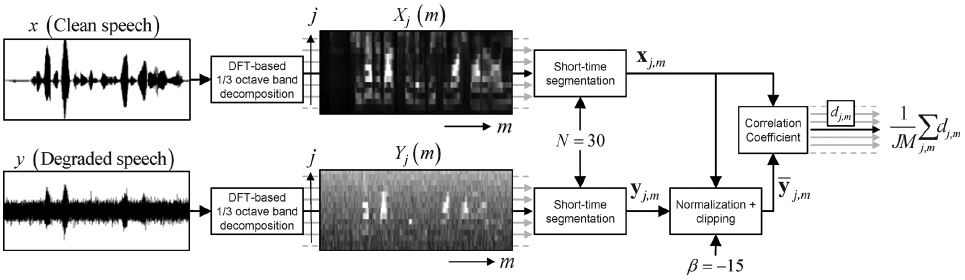
\includegraphics[width=\linewidth]{Features/images/stoi_blocks_diagram}
    \caption{STOI flow diagram}\label{fig:stoi_blocks_diagram}
    \source{Adapted from \cite{5495701}}
\end{figure}

The STOI algorithm structure is demonstrated in 
the blocks diagram shown in Figure\;\ref{fig:stoi_blocks_diagram}. 

The short-time temporal envelop of the degraded
speech \(Y_{_{j,m}}\) is clipped and normalized
before the extraction of the correlation coefficient
with the short-time temporal envelop of the
clean speech \(X_{_{j,m}}\).
This clipped normalized version then be:
\begin{align}
    \mathcal{Y}[n] & = \min\Bigg\{ 
            \frac{||X_{_{j,m}}||}{||Y_{_{j,m}}||} Y_{_{j,m}}[n]
            ,\; (1+10^{\sfrac{-\beta}{20}})X_{_{j,m}}[n]
        \Bigg\}
\end{align}

Thus, the correlation coefficient can be expressed as the
distance given in Equation\;\ref{eq:stoi_correl}.
\begin{align}\label{eq:stoi_correl}
    d_{_{j,m}} & = \frac{
            (X_{_{j,m}}-\bar{X}_{_{j,m}})^{tr} 
            \cdot (\mathcal{Y}_{_{j,m}}-\bar{\mathcal{Y}}_{_{j,m}})
        }
        {
            ||X_{_{j,m}}-\bar{X}_{_{j,m}}||
            \cdot ||\mathcal{Y}_{_{j,m}}-\bar{\mathcal{Y}}_{_{j,m}}|| 
        }
\end{align}
Also, defining the intermediate intelligibility measure, 
Equation\;\ref{eq:stoi_correl}, it stands for the
\(m^{th}\) time frame. Extending it to form
a definition for the entire signal,
we can take the average of \(d_{_{j,m}}\)
as in Equation\;\ref{eq:stop_dist_avg}.

\begin{align}\label{eq:stop_dist_avg}
    d & = \frac{1}{JM} \sum_{j,m} d_{_{j,m}}
\end{align}

Where \(J\) presents the total number of one-third octave bands,
and the averaging overlaps \(M\) number of time frames.

\subsection{PESQ -- Perceptual Evaluation of Speech Quality}
PESQ\cite{941023} is a measuring method adopted by 
the ITU (International Telecommunication Union, ITU-T P.862) to
test the speech quality of telephony and mobile stations.

This measuring metric evolved from different previous 
measuring techniques such as Bark Spectral Distortion (BSD),
Perceptual Analysis Measurement System (PAMS),
and Perceptual Speech Quality Measure (PSQM).

The motivation behind the development of the PESQ metric
was the need to assess the speech quality in an E2E
communication channel that considers 
the entire link rather than particular parts.

The evaluation of a speech signal quality by PESQ
follows the MOS (Mean Opinion Scores) scoring model, where
the actual speech quality is ranked in-between 1 to 5 
by a group of listeners. The MOS is a subjective measure,
while the PESQ is an objective measure.

Figure \ref{fig:pesq_blocks_diagram} shows the data flow
of the PESQ computation for a predicted signal, with respect to the
clean reference.

\begin{figure}[H]
    \centering
    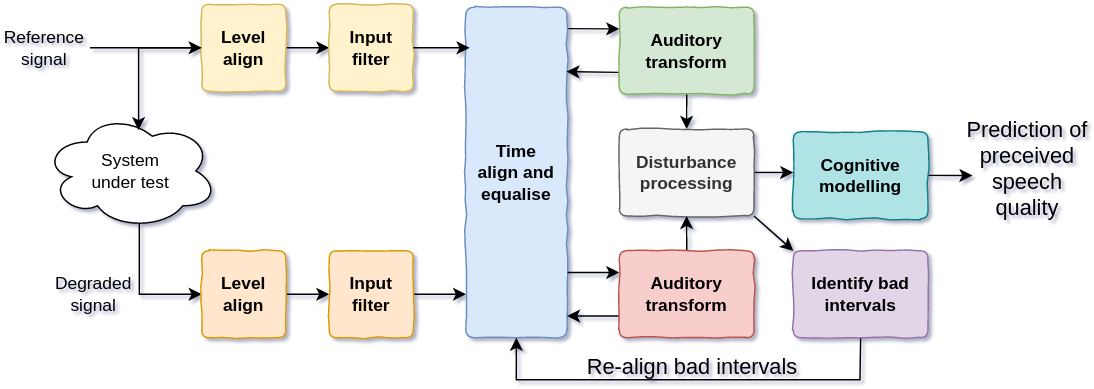
\includegraphics[width=0.85\linewidth]{Features/images/pesq_blocks_diagram_new}
    \caption{PESQ Algorithm Blocks Diagram}\label{fig:pesq_blocks_diagram}
    \source{Adapted from PESQ paper\cite{941023} and redesigned}
\end{figure}

\section{ASR Metrics}
\subsection{WER -- Word Error Rate}
WER\cite{KLAKOW200219} metric is probably the most used evaluation
technique for speech recognition systems.

Evaluation of this metric occurs at the ASR engine's output, 
where the predicted text is segmented into sentences. 
Each word in the predicted
text is then matched with its counterpart in the 
annotated reference transcript. 
The sum of mismatches between a predicted sentence and the reference, 
divided by the total counted words in the reference, indicates the WER.

However, in some cases, the predicted sentences differ in size compared
to the reference. Therefore, special care for \emph{Insertions}
and \emph{Deletions} should be carried out as well, without neglecting
the detected \emph{Substitutions}.

The WER is described by:
\begin{align}
    WER & = \frac{S + D + I}{N}
\end{align}

Where \(N\) is the total count of words in the reference,
and \(S,D,I\) are the number of \emph{Substitutions} (wrong word detection),
\emph{Deletions} (Omitting words),
and \emph{Insertions} (Wrong words insertions).

\subsection{CER -- Character Error Rate}
CER is another metric with some similarities to the 
WER evaluation metric but with a narrower resolution.
The change in resolution is due to comparing characters instead of words.
The same rules of \emph{Substitutions}, \emph{Deletions}, and \emph{Insertions}
apply, and therefore, the calculation of the CER is the same:
\begin{align}
    CER & = \frac{S + D + I}{N}
\end{align}

In many cases, the CER\cite{_isword} is a complementary 
measuring metric to the WER
metric.
This extra measure shines especially 
when there is a need to get a full perspective 
with a greater differentiation capability of the 
\emph{Substitutions} in the complete sentence 
of the suggested predicted transcript,
 also known as the hypothesis. 
While WER counts a mismatch between the reference and the predicted 
word, even in cases where only single characters or worse, 
punctuation marks are not correctly placed, CER can lead to 
more accurate grading per word.

\section{Hardware Metrics}
% \subsection{Computation time}
% \subsection{Utilization Ratio}
\subsection{Power Estimation}
Electrical circuits, components, and systems require power to function.
The amount of power a device consumes from the power sources is subject 
to various parameters and mainly describes the rate of energy delivery 
from the source to the device or vice versa.

Due to the nature of conducting materials, 
whenever an electrical potential is applied
between the conductor's terminals, 
electrical current goes through the conductor.
The current that flows
in the system feeds the different components with energy. 
However, the total supplied energy is not purely consumed over time, 
and some energy is lost and wasted due to power dissipation.

Power dissipation is a side effect of a conductors' resistive nature, 
which "resists" the transition of current through it.
As a result, part of the energy in the system is converted 
to heat energy.

Since dissipated power is a waste of energy it is also 
considered as one of the main causes 
to electronic systems' performance degradation at high temperatures.
Therefore, engineers want to mitigate 
as much as possible any dissipated power that
is not used for the main functionality of the system. % but dissipated and converted to heat.
For that end, power analysis is crucial in any system 
design phase to ensure efficiency and correctness while maintaining 
robustness over time and under different working conditions.

Electrical circuit power dissipation depends on many arguments. % mainly when speaking of digital logic designs. 
However, in general, it can be modeled 
accurately according to three scenarios divided into two main groups:
\begin{enumerate}
    \item Static Power
    \begin{itemize}
        \item Intrinsic Leakage Power
    \end{itemize}
    \item Dynamic Power
    \begin{itemize}
        \item Internal Power
        \item Switching Power
    \end{itemize}
\end{enumerate}

\subsubsection{Intrinsic Leakage Power}
Leakage power is the power that dissipates due to the 
structure of a CMOS device, 
where a thin layer of metal oxide isolates
between the semiconductor material and the
gate metal and thus forming a capacitor. 
Leakage power dissipates statically regardless of the CMOS 
device state, 
whether it is the active state or the off state (idle).

\begin{figure}[H]
    \centering
    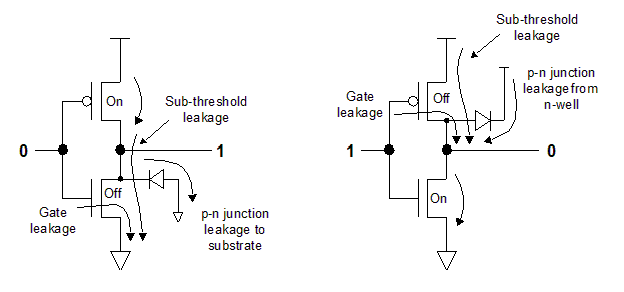
\includegraphics[width=0.75\linewidth]{Features/images/leak_power_schem}
    \caption{Leakage Power Illustration}\label{fig:leak_power_schem}
    \source{Adapted from Synopsys PrimePower Suit documentation\cite{lowpowerSoc}}
\end{figure}

Figure \ref{fig:leak_power_schem} describes three current leakages,
the reverse bias current of the diode (p-n junction), sub-threshold current leakage, and
the gate leakage.

With the recent advancement in process technologies, 
CMOS devices are minimized in size, 
but the leakage power is increasing as a side effect.
\begin{figure}[H]
    \centering
    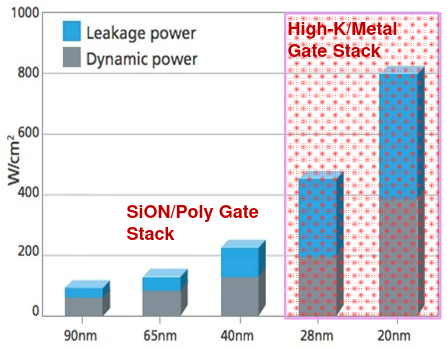
\includegraphics[width=0.55\linewidth]{Features/images/leak_vs_nm}
    \caption{Leakage Power vs. Process Technology}\label{fig:leak_vs_nm}
    \source{Adapted from Soitec FinFet presentation\cite{processnodeleak}}
\end{figure}
The overall leakage power is a function 
of the total number of voltage sources and their voltage levels, 
the physical dimensions of the CMOS device, 
and the threshold value set to switch between on-off states.
% \begin{align}\label{eq:}
%     P_{leak} & = \mathcal{F} (V_{_{DD}}, V_{_{th}}, \frac{\mu_{n}\varepsilon_{ox} W}{L})
% \end{align}

\subsubsection{Internal Power}
A CMOS device is a formation of two complementary MOS transistors,
a p-type and an n-type, formed together as a symmetrical
pair unit. 
Internal power dissipation happens due to the structure of
CMOS devices. 
Whenever a transition at the CMOS gate occurs, 
both the NMOS and the PMOS drivers are active for a 
relatively small duration of time. As a result, 
a short circuit is formed directly from the power rail to the ground. 
Although not lasting for long periods of time, 
the amount of internal dissipated power in highly toggled 
designs becomes significant over time. 
To minimize the internal dissipated power, 
or in other words, minimizing the time duration where 
both devices are active and current flows from \(V_{dd}\) to GND, 
the transition times (both rising and falling) are set to be very fast.

\begin{figure}[H]
    \centering
    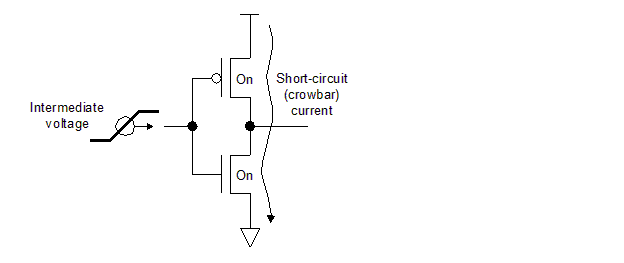
\includegraphics[width=0.75\linewidth]{Features/images/int_power_schem}
    \caption{Internal Power Illustration}\label{fig:int_power_schem}
    \source{Adapted from Synopsys PrimePower Suit documentation\cite{lowpowerSoc}}
\end{figure}

\subsubsection{Switching Power}
Switching power is the power dissipated as a result 
of charging and discharging loads during transitions. 
MOS devices introduce capacitance at their input gates 
due to their structure. 
Thus, whenever a low-to-high transition at the output occurs, 
the driver pushes the current to charge the capacitive 
load in order to set the desired logic level voltage. 
Likewise, the load capacitance discharge and sink into the 
device through the PMOS transistor to the ground 
for a high-to-low transition at the output. 
As a result, the charging and discharging currents 
eventually dissipate and are not delivered to the external load.

\begin{figure}[H]
    \centering
    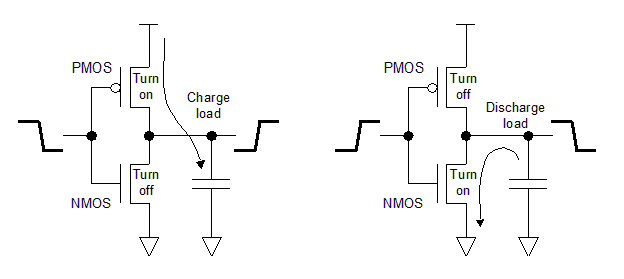
\includegraphics[width=0.75\linewidth]{Features/images/sw_power_schem}
    \caption{Switching Power Illustration}\label{fig:sw_power_schem}
    \source{Adapted from Synopsys PrimePower Suit documentation\cite{lowpowerSoc}}
\end{figure}